\documentclass[11pt, oneside]{article}   	% use "amsart" instead of "article" for AMSLaTeX format
\usepackage{geometry}                		% See geometry.pdf to learn the layout options. There are lots.
\geometry{letterpaper}                   		% ... or a4paper or a5paper or ... 
%\geometry{landscape}                		% Activate for for rotated page geometry
%\usepackage[parfill]{parskip}    		% Activate to begin paragraphs with an empty line rather than an indent
\usepackage{graphicx}				% Use pdf, png, jpg, or eps� with pdflatex; use eps in DVI mode
								% TeX will automatically convert eps --> pdf in pdflatex		
\usepackage{amssymb}
\usepackage{amsmath}
\usepackage{parskip}
\usepackage{color}
\usepackage{hyperref}

\title{Cauchy integral theorem}
%\author{The Author}
%\section{}
%\subsection*{}
\date{}							% Activate to display a given date or no date

\graphicspath{{/Users/telliott_admin/Dropbox/Tex/png/}}
% \begin{center} 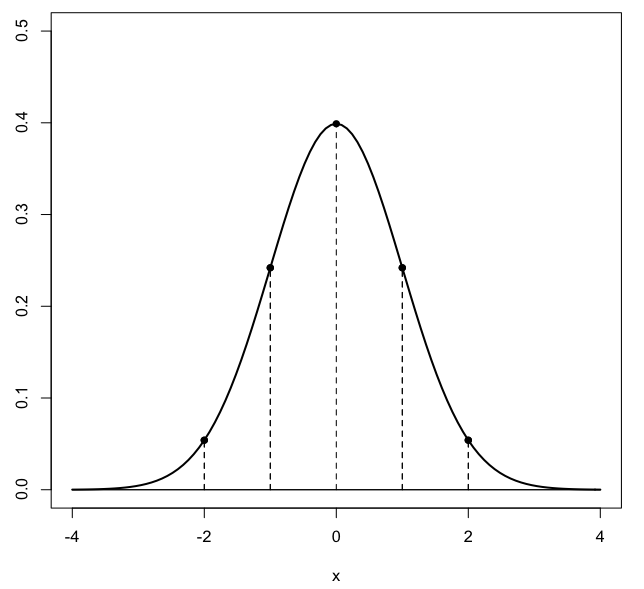
\includegraphics [scale=0.4] {gauss3.png} \end{center}
\begin{document}
\maketitle
\Large

\subsection*{Cauchy' First Integral Theorem}

Cauchy's first theorem says that the integral of an analytic function over a closed path is equal to zero (when the enclosed region is without a singularity).
\[ \oint_C f(z) \ dz = 0 \]
This will turn out to be a consequence of Green's Theorem, which I've written about a lot before.  Let
\[ z = x + i y \]
\[ dz = dx + i dy \]
\[ z = f(x,y) = u(x,y) + iv(x,y) \]
Our integral is
\[ \oint_C z \ dz = \int (u(x,y) + iv(x,y)) \ (dx + i dy) \]
\[ =  \oint_C u(x,y) \ dx - \int v(x,y) \ dy + i \int v(x,y) \ dx + i \int u(x,y) \ dy \]
As before, because we are moving along a curve there is a relationship between $x$ and $y$, so we can either express that relationship or parametrize the curve.  In any case, these become integrals in a single variable.  We remove extra $(x,y)$ notation:
\[ =  \oint_C u \ dx - \int v \ dy + i \int v \ dx + i \int u \ dy \]

\subsection*{proof of Cauchy 1}
Back in vector calculus we proved Green's theorem, which says that for two real functions of $x$ and $y$:  $M(x,y)$ and $N(x,y)$:
\[ \oint_C M dx + N dy = \iint_R (\frac{\partial N}{\partial x} - \frac{\partial M}{\partial y}) \ dx \ dy \]
Back then, $M$ and $N$ were components of a vector field $\mathbf{F}$ and we wrote the shorthand for curl:
\[ = \iint_R \nabla \times \mathbf{F} \ dA\]
but the important thing is that they are real functions of two variables $f: \mathbb{R}^2 \rightarrow \mathbb{R}^1$.

In terms of $u$ and $v$ we have for the real part of Cauchy's Theorem that $M=u$ and $N = -v$ (notice the minus sign!).  

So:
\[ \oint u \ dx - \oint v \ dy = \iint_R (-\frac{\partial v}{\partial x} -  \frac{\partial u}{\partial y}) \ dx \ dy \]
\[ = - \iint_R (v_x + u_y) \ dx \ dy \]
But, according to the CRE
\[ u_y = -v_x \]
Hence, this integral is zero.

For the imaginary part:
\[ \oint v \ dx + \oint u \ dy =  \iint_R (\frac{\partial u}{\partial x} - \frac{\partial v}{\partial y}) \ dx \ dy \]g
\[ =  \iint_R (u_x - v_y) \ dx \ dy \]
But, again, according to the CRE
\[ u_x = v_y \]
So the integral for the imaginary part is also zero, and thus the whole thing is zero as well:
\[ \oint u \ dx - \oint v \ dy + i \oint v \ dx + i \oint u \ dy = 0 \]

Remember how important it was (for Green's theorem) that the function being integrated be defined everywhere in the region.  For example, it is \emph{not} true that

\[ \oint_C \frac{1}{z} \ dz = 0 \]

if the curve $C$ includes the origin, but it \emph{is} true otherwise.  A simple demonstration for the former case is the unit circle centered at the origin.  We write
\[ z = r e^{i\theta} \]
\[  \frac{dz}{d\theta} = r i e^{i\theta} = iz \]
Hence
\[ \oint_C \frac{1}{z} \ dz = \oint_C \frac{1}{z} \ iz \ d \theta \]
\[ = i   \oint_C  d \theta = 2 \pi i \]

\end{document}  